\section{Auswertung}
\label{sec:Auswertung}
Der Selektivverstärkers soll zunächst untersucht werden.
Dazu wird die Frequenz und die dazugehörige Ausgangsspannung $U_A$ im Frequenzbereich von 20 bis 40 $\si{\kilo\hertz}$ aufgenommen.
Die Messpaare sind in der Tabelle \ref{tab:Messergebnisse} zu finden.
Zudem ist die Filterkurve in Abbildung \ref{fig:filterkurve} zu sehen.
Aus der Abbildung \ref{fig:filterkurve} ist ein Spannungshoch im Frequenzbereich von 22.5 und 25 $\si{\kilo\hertz}$ zu erkennen.
Weitere Aussagen können aus den Messergebnissen nicht getroffen werden.

\begin{table}
  \centering
  \caption{Messergebnisse für die Filterkurve des Selektivverstärkers.}
  \label{tab:Messergebnisse}
  \begin{tabular}{c c}
    \toprule
    {$U_A$ [$\si{\milli\volt}$]} & {$\nu$ [$\si{\micro\ampere}$]}\\
    \midrule
    \input{tabelle_selektiv.txt}
    \bottomrule
  \end{tabular}
\end{table}

\begin{figure}
  \centering
  \caption{Filterkurve des Selektivverstärkers.}
  \label{fig:filterkurve}
  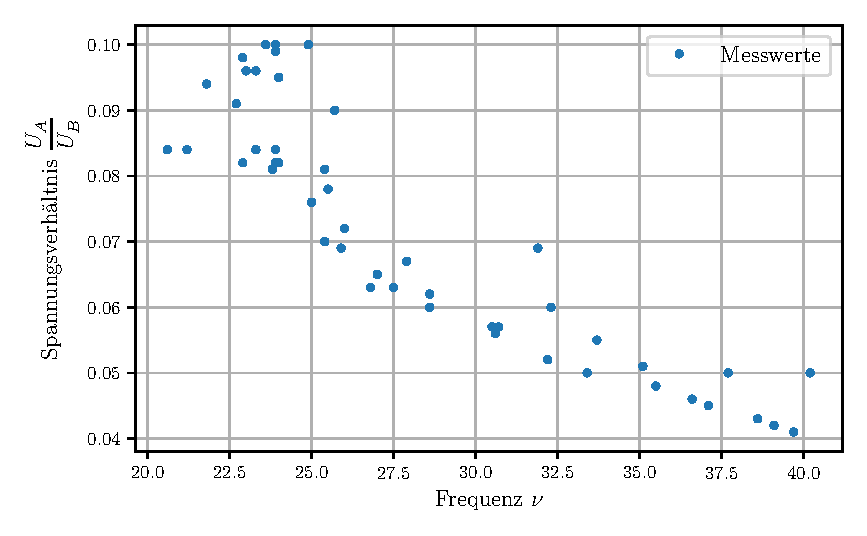
\includegraphics{content/filterkurve.pdf}
\end{figure}

Die Suszeptibilitäten $\chi$ der beiden Stoffe sollen mithilfe der Messwerte aus Tabelle \ref{tab:Messwerte} bestimmt werden.
Dabei werden die Formeln \ref{eqn:chi_r} und \ref{eqn:chi_u} verwendet.
In der Tabelle \ref{tab:Suszeptibilität_Praxis} sind die Ergebnisse zu finden.

\begin{table}
  \centering
  \caption{Messergebnisse zur Bestimmung der Suszeptibilitäten.}
  \label{tab:Messwerte}
  \begin{tabular}{c c c c c}
    \toprule
    {Stoff} & {$U_{\text{Br ohne}}$ [$\si{\milli\volt}$]} & {$U_{\text{Br mit}}$ [$\si{\milli\volt}$]} & {$R_{3 ohne}$ [$\si{\milli\ohm$]} &{$R_{3 mit}$ [$\si{\milli\ohm$]}\\
    \midrule
    $\ce{Dy2O3}$ & 0.9 & 3.7 & 2964.5 & 1690.0\\
              &1.3 & 3.92 & 2981.0 & 1530.0\\
              &1.2 & 4.2 & 3059.0 & 1485.5 \\
    $\ce{Gd2O3}$ &2.0 & 4.05 & 3136.5 & 2360.0 \\
              &2.15 & 4.07 & 3157.5 & 2398.0 \\
              &2.1 & 3.85 & 3137.0 & 2381.0 \\
    \bottomrule
  \end{tabular}
\end{table}

\begin{table}
  \centering
  \caption{Suszeptibilitäten aus den Messergebnissen.}
  \label{tab:Suszeptibilität_Praxis}
  \begin{tabular}{c c c}
    \toprule
    {Stoff} & {$\chi_U$} & {$\chi_R$} \\
    \midrule
    $\ce{Dy2O3}$ & -7.3832 $\pm$ 0.5442 & 0.1219 $\pm$ 0.00633 \\
    $\ce{Gd2O3}$ & -3.8715 $\pm$ 0.05117 & -3.8715 $\pm$ 0.05117 \\
    \bottomrule
  \end{tabular}
\end{table}

Die Suszeptibilitäten aus den Messergebnissen werden mit dem Theoriewert verglichen.
Dieser wird mithilfe der Formel \ref{eqn:sus_theo} bestimmt.
In Tabelle \ref{tab:Proben} ist jeweils die Dichte $\rho$, Masse $m$, Länge $l$, molare Masse $M$ und der reale Querschnitt $Q$ der beiden Proben zu finden, die für die Berechnung benötigt werden.
Der reale Querschnitt $Q$ wird mit der Formel \ref{eqn:qreal} ermittelt.

\begin{table}
  \centering
  \caption{Werte der Proben.}
  \label{tab:Proben}
  \begin{tabular}{c c c c c c }
    \toprule
    {Stoff} & {$\rho$ [$\si{\gram\per\centimetrecubed}$]} & {$m$ [$\si{\gram}$]} & {$l$ [$\si{\centimetre}$]} & {$M$ [$\si{\gram\per\mole}$]} & {$Q$ [$\si{\centimetresquared}$]}\\
    \midrule
    $\ce{Dy2O3}$ & 7.8 & 15.1 & 17.3 & 372.9982 & 0.1119\\
    $\ce{Gd2O3}$ & 7.4 & 14.08 & 17.5 & 2.0 & 362.4982 & 0.1087\\
    \bottomrule
  \end{tabular}
\end{table}

\begin{table}
  \centering
  \caption{Quantenzahlen und Landé-Faktoren.}
  \begin{tabular}{c c c c c }
    \toprule
    {Stoff} & {$L$} & {$S$} & {$J$} & {$g_J$}\\
    \midrule
    $\ce{Dy2O3}$ & 5 & 2.5 & 7.5 & 1.33\\
    $\ce{Gd2O3}$ & 0 & 3.5 & 3.5 & 2.0\\
    \bottomrule
  \end{tabular}
\end{table}

\begin{table}
  \centering
  \caption{Vergleich der Suszeptibilitäten.}
  \begin{tabular}{c c c c c c}
    \toprule
    {Stoff} & {$\chi_T$} &{$\chi_U$} & {$\frac{\chi_T - \chi_U}{\chi_T}$} & {$\chi_R$} & {$\frac{\chi_T - \chi_R}{\chi_T}$}\\
    \midrule
    $\ce{Dy2O3}$ & 2.1327 & 0.08688 $\pm$ 0.0048 & 0.9593 & 7.3832 $\pm$ 0.5442&  -2,4619\\
    $\ce{Gd2O3}$ & 1.1573 &  0.06075 $\pm$  0.00391 & 0.9475 &3.8715 $\pm$ 0.05117 & -2.3453 \\
    \bottomrule
  \end{tabular}
\end{table}